\section{Constat \& Objectif du stage}
Au sein de la direction Delivery, les équipes de développement travaillent avec les équipes d’exploitation selon des principes devops.
Pour cela, elles disposent d’un outillage self-service (Katana) pour, entre autres,
livrer leurs applications et les déployer sur les différentes plateformes (usine, recette, pré-production, production).
A date, cet outillage supporte les activités de plus de 150 applications, sur plus de 1500 plateformes.

Pour utiliser cet outillage,
les équipes de développement génèrent pour chaque version de leurs applications une note de livraison (lexique.\ref{lexi:delivery_note}) qui porte l’ensemble des informations utiles associées
(identifiant et emplacement des livrables applicatifs, moyens de tester le bon fonctionnement, pré-requis et instructions d’installation, etc).
Ce document prend la forme d’un fichier structuré (JSON).

Objectif de ce projet est de créer une application web (IHM + API REST) pour manipuler les notes de livraison Katana, qui permet de :

\begin{itemize}
 \item gérer l'objet NDL de manière plus simple qu'avec Nexus/filesystème;
 \item éviter les tableaux de suivi, type notes d'installation, tableaux de dépendances... qui sont édités manuellement;
 \item fédérer certaines fonctionnalités (extraction d'information, identification des packages à installer sur une plateforme...) par rapport aux scripts bash/groovy/perl/ruby....
 \item outiller le suivi du cycle de vie des versions par rapports aux informations remontées par les outils de l'usine logicielle et Katana.
\end{itemize}

L’application devra être légère, dynamique et facilement évolutive, et non-contraignante pour les équipes.

Le but est de fiabiliser le processus de livraison et de mise en production des applications.

Le stage contient, dans une démarche itérative :
\begin{itemize}
  \item le recueil des besoins auprès des utilisateurs (passé un cahier des charges initial);
  \item La conception de l’application en accord avec le responsable d’équipe :
  \begin{itemize}
    \item Conception des pages, des services REST et de l’application dynamique sous-jacente;
    \item Modélisation des données nécessaires à l’application, le cas échéant.
  \end{itemize}
  \item Le développement de l’application;
  \item La documentation de l’application;
  \item Le rapport des activités au responsable de l’équipe.
\end{itemize}

\begin{figure}[ht]
 \centering
 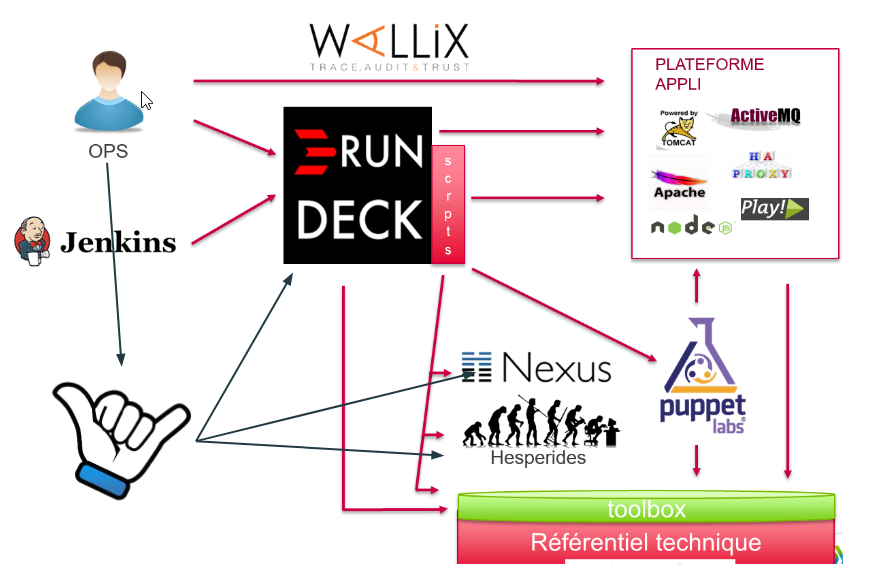
\includegraphics[width=0.8\textwidth]{dn_rider_position}
 \caption{Dn Rider}
\end{figure}

\clearpage
